%! Author = Antonio Lobo
%! Date = 30/10/2024

\section{Reduction Methods}
In this section, we briefly describe reduction techniques employed for instance-based learning. We use a simple 2D dataset ($D_1$) for illustrative purposes, shown in \textbf{Figure} \ref{fig:2dDatasetReduction}.
\begin{figure}[ht]
	\centering
	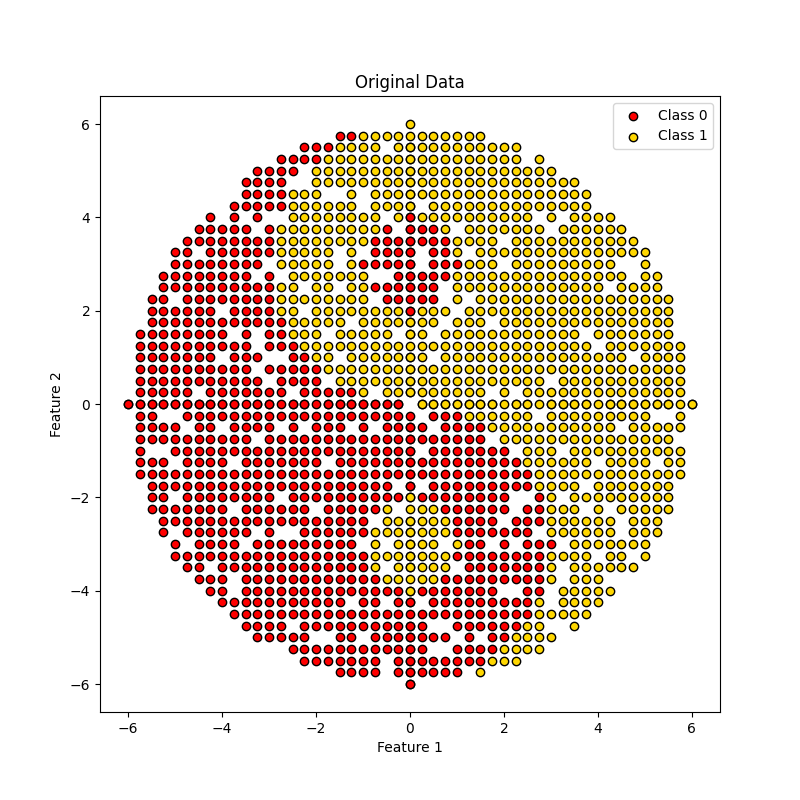
\includegraphics[width=\textwidth]{figures/2dDataset} % Adjust the path and size as needed
	\caption{2D example dataset}
	\label{fig:2dDatasetReduction}
\end{figure}

\subsection{GCNN}
\subsection{EENTH}
\subsection{DROP3}
In this subsection, we describe the basic concepts of the third method in the Decremental Reduction Optimization Procedure (DROP) family, as presented in Section 3 of Wilson et al. \cite{wilson2000reduction}. Although we will not delve into every detail, we describe the main ideas of the algorithm and illustrate them on $D_1$.

\begin{enumerate}
	\item \textbf{Remove noise}: The first step is to remove noisy instances using Edited Nearest Neighbor (EEN) \cite{wilson1972asymptotic}, where any instance misclassified by its \( k \)-nearest neighbors is removed. The outcome of applying this technique is shown in \textbf{Figure} \ref{fig:2dEEN}, where noise has been removed. We denote the reduced dataset as $ T \subseteq D_1 $.
	\begin{figure}[ht]
		\centering
		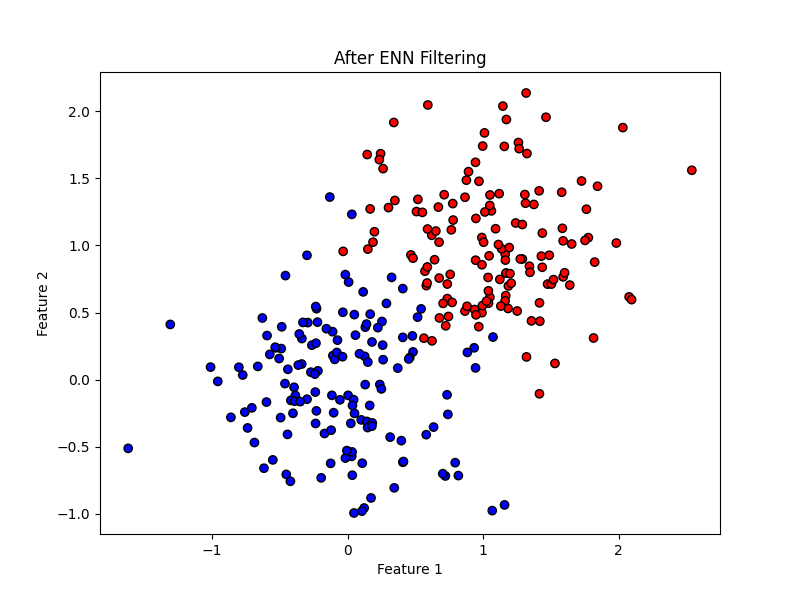
\includegraphics[width=\textwidth]{figures/2dEEN} % Adjust the path and size as needed
		\caption{Example of EEN noise removal}
		\label{fig:2dEEN}
	\end{figure}
	
	\item \textbf{Sort points}: The next step is to prioritize removing points that are farthest from the decision boundary. For each point $ x_i \in S $ with class $ y_i $, we compute the distance to the nearest point with a different class, denoted as $ x_j \in D $ such that $ y_j \neq y_i $ and $ \nexists x_k : |x_k - x_i| < |x_j - x_i| \land y_i \neq y_k $.
	
	\item \textbf{Delete points}: Let $ S = T $. Starting with the points farthest from the boundary, we check if any associated points (points that have $ x_i $ as a neighbor) $ a_j $ receive more votes for their correct class with $ x_i $ as a neighbor (denoted as $ \text{with} $) or if they would be classified correctly if $ x_i $ were removed (denoted as $ \text{without} $). If $ \text{without} > \text{with} $, we remove $ x_j $ from $ S $, resulting in $ S' = S \setminus \{x_j\} $.
	
	\item \textbf{Selecting neighbors}: A key distinction between DROP1 and DROP2 is that DROP1 considers neighbors for $ a_j $ from the whole dataset $ T $, whereas DROP2 does not. Wilson et al. \cite{wilson1972asymptotic} do not specify this factor explicitly; therefore, we test both options, as DROP3 seems to be built on top of DROP2. A comparison of these methods is shown in \textbf{Figures} \ref{fig:DROP3Reduciendo} and \ref{fig:DROp3Total}.
	
	\begin{figure}[ht]
		\centering
		\begin{minipage}{0.45\textwidth}
			\centering
			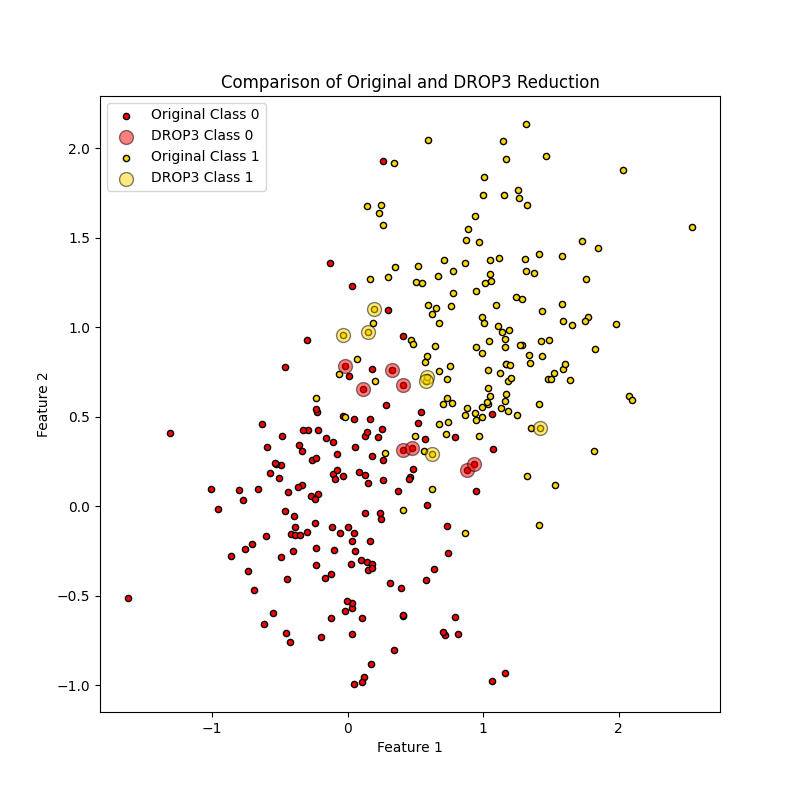
\includegraphics[width=\textwidth]{figures/DROP3Reduciendo} % Adjust path and file name
			\caption{Effect of DROP3 reducing the dataset as DROP1}
			\label{fig:DROP3Reduciendo}
		\end{minipage}\hfill
		\begin{minipage}{0.45\textwidth}
			\centering
			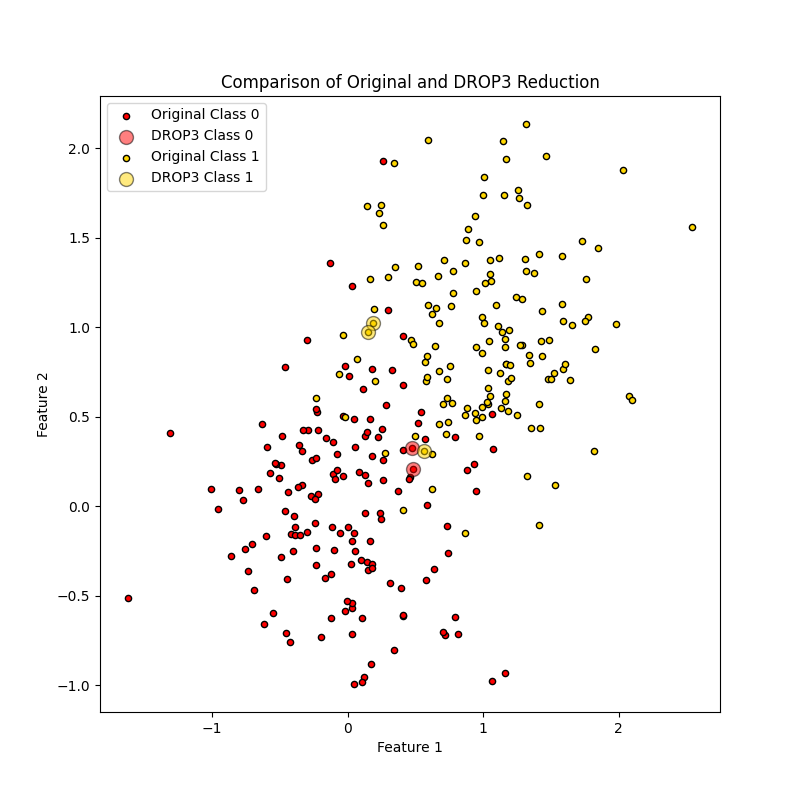
\includegraphics[width=\textwidth]{figures/DROP3Total} % Adjust path and file name
			\caption{Effect of DROP3 using $T$ as DROP2}
			\label{fig:DROp3Total}
		\end{minipage}
	\end{figure}
	
\end{enumerate}
